\documentclass%
%[handout]
{beamer}
% % % % % % % %
% % % % % % % %
% % % % % % % %
%IMPORTANT
%compiles with 
%pdflatex -shell-escape 
%IMPORTANT
% % % % % % % %
% % % % % % % %
% % % % % % % %
\mode<presentation>
{
\useinnertheme{rounded}
\useoutertheme{infolines}
\usecolortheme{orchid}
\usecolortheme{whale}
}

\usepackage[english]{babel}
\usepackage[latin1]{inputenc}
\usepackage[all,cmtip]{xy}
\usepackage{times}
\usepackage[T1]{fontenc}
\usepackage{../example-templates}
\usepackage{../pstricks-commands}
\usepackage{cancel}

\usepackage{auto-pst-pdf}
\usepackage{pst-plot}
%\usepackage{pstricks-add} 

% Or whatever. Note that the encoding and the font should match. If T1
% does not look nice, try deleting the line with the fontenc.

\graphicspath{{../../modules/}}

\newtheoremstyle{partialproof}{3pt}{3pt}{}{}{}{.}{.5em}{}
\theoremstyle{partialproof} \newtheorem{partialproof}[theorem]{Proof.}
%\DeclareMathOperator{\diff}{d}
\newcommand{\diff}{\text{d}}
\setbeamertemplate{navigation symbols}{}

\includeonlylecture{1}

\newcommand{\lect}[3]{
  \date{#1}
  \lecture[#1]{#2}{#3}
}

\setbeamertemplate{footline}
{
  \leavevmode%
  \hbox{%
  \begin{beamercolorbox}[wd=.333333\paperwidth,ht=2.25ex,dp=1ex,center]{author in head/foot}%
    \usebeamerfont{author in head/foot}\insertshortauthor
  \end{beamercolorbox}%
  \begin{beamercolorbox}[wd=.333333\paperwidth,ht=2.25ex,dp=1ex,center]{title in head/foot}%
    \usebeamerfont{title in head/foot}\insertshorttitle
  \end{beamercolorbox}%
  \begin{beamercolorbox}[wd=.333333\paperwidth,ht=2.25ex,dp=1ex,center]{date in head/foot}%
    \usebeamerfont{date in head/foot}\insertshortdate{}
  \end{beamercolorbox}}%
  \vskip0pt%
}

% If you have a file called "university-logo-filename.xxx", where xxx
% is a graphic format that can be processed by latex or pdflatex,
% resp., then you can add a logo as follows:

%\pgfdeclareimage[height=0.8cm]{logo}{bluelogo}
%\logo{\pgfuseimage{logo}}

\begin{document}

\AtBeginLecture{%

\title[\insertlecture]{FreeCalc}
\subtitle{\insertlecture}
\author[FreeCalc]{}
\institute[UMass Boston]{University of Massachusetts Boston}
\date{\insertshortlecture}
\begin{frame}
  \titlepage
\end{frame}
}%

% begin lecture
\lect{\today}{Sample}{1}
%% begin module curve-sketching-guidelines
\begin{frame}
\frametitle{Guidelines for Sketching a Curve}
The following items are to be considered when drawing a curve. \alert<2>{Not every item is relevant to every function.}
\begin{enumerate}
\item  Determine the domain of the function.
\item  Depending on availability, use computer software to plot. 
\item  \alert<2>{Compute $x,y$ intercepts.}
\item  \alert<2>{Determine symmetries, periodicity.}
\item  \alert<2>{Compute asymptotes - vertical, horizontal, {\color{gray} optional - slanted}.}
\item  Compute intervals of increase or decrease.
\item  Compute local and global maxima and minima.
\item  Compute concavity and points of inflection.
%\item  Sketch the curve
\end{enumerate}
\end{frame}

\begin{frame}[t]
\begin{enumerate}
\item  \alert<3>{Domain}
\begin{itemize}
\item  Find the domain of the function.  
\item  Remember the two restrictions: no dividing by $0$, and no taking the even root of a negative number.
\end{itemize}
\item<2-> You can use computer software to plot your function.
\begin{itemize}
\item<3-> Most computer software will ask you to specify the \alert<3>{domain of the function} explicitly.
\item<4-> Some software may be able to determine the (implied) domain of your function.
\item<5-> Software may not be always available (example: Calculus I exams).
\end{itemize} 
\end{enumerate}
\end{frame}


\begin{frame}[t]
\begin{enumerate}
\setcounter{enumi}{2}
\item  Intercepts
\end{enumerate}
\begin{itemize}
\item  Find the intercepts of the function.
\item  $f(0)$ is the $y$-intercept.
\item  To find the $x$-intercepts, set $y = 0$ and solve for $x$.
\item  You can sometimes skip this step if the equation is too difficult to solve.
\end{itemize}
\end{frame}


\begin{frame}[t]
\begin{enumerate}
\setcounter{enumi}{3}
\item  Symmetry, Periodicity
\end{enumerate}
\begin{itemize}
\item<1-| alert@2>  \alert<handout:1| 0>{If $f(-x) = f(x)$ for all $x$, then $f$ is even.}
\item<1-| alert@3>  \alert<handout:2| 0>{If $f(-x) = -f(x)$ for all $x$, then $f$ is odd.}
\item<1-| alert@4>  \alert<handout:3| 0>{If there is some number $p$ such that $f(a+p) = f(a)$ for all $a$, then $f$ is called periodic.  The smallest such $p$ is called its period.}
\end{itemize}
\begin{center}

\ \only<handout:1| -2>{%
\uncover<2>{%
\psset{xunit=1cm, yunit=1cm}
\begin{pspicture}(-1.7,-1.5)(1.7,2.5721)
\tiny 
\psaxes[ticks=none, labels=none]{<->}(0,0)(-1.7,-1.5)(1.7,2.5721)
\psLabels{1.7}{2.5721}
\psXTickWithLabel{-1}{$-1$}
\psXTickWithLabel{1}{$1$}
%Function formula: -2 x^{2}+x^{4} 
%\rput(1,3){$y=-2 x^{2}+x^{4}$} 
\psFullDot{-1.5}{0.5625}
\psFullDot{1.5}{0.5625}
\rput[r](-1.6, 0.5625){$(-1.5, f(1.5))$}
\rput[l](1.6, 0.5625){$(1.5, f(1.5))$}
\psline{<->}(-1.4, 0.5625)(1.4, 0.5625)
\psFullDot{-1}{-1}
\psFullDot{1}{-1}
\rput[rt](-1.1, -1){$(-1, f(1))$}
\rput[lt](1.1, -1){$(1, f(1))$}
\psline{<->}(-0.9, -1)(0.9, -1)

\psplot[linecolor=\psColorGraph, plotpoints=1000]{-1.7}{1.7}{x 4 exp x 2 exp -2 mul add }
\end{pspicture}
}}%
\only<handout:2| 3>{%
\psset{xunit=1cm, yunit=1cm}
\begin{pspicture}(-3.2,-2)(3.2,2)
\tiny 
\psaxes[ticks=none, labels=none]{<->}(0,0)(-3.2,-2)(3.2,2)
\psLabels{3.2}{2}
\psXTickWithLabel{1}{$1$}
\psXTickWithLabel{-1}{$-1$}
%Function formula: \sin{}x 
\psplot[linecolor=\psColorGraph, plotpoints=1000]{-3}{3}{x 57.29578 mul sin }
%Function formula: \sqrt{- x^{2}+17080660249/10000000000} 
\psplot[arrows=->, plotpoints=1000]{-1.3068}{0.92}{1.70807 x 2 exp -1 mul add sqrt }
%Function formula: -\sqrt{- x^{2}+17080660249/10000000000} 
\psplot[arrows=->, plotpoints=1000]{-1.3068}{-1.08}{1.70807 x 2 exp -1 mul add sqrt -1 mul}
\psFullDot{1}{0.841471}
\rput[lt](1,0.741471 ){$(1, f(1))$}
\psFullDot{-1}{-0.841471}
\rput[t](-1,-1.05 ){$(-1, -f(1))$}
\rput[lb](1.5, 1.1){$y=f(x)$}
\end{pspicture}
}%

\only<handout:3| 4->{%
\psset{xunit=0.75cm, yunit=0.75cm}
\begin{pspicture}(-6,-0.7)(6,4.5)
\tiny 
\psaxes[ticks=none, labels=none]{<->}(0,0)(-6,-0.7)(6,4.5)
\psLabels{6}{4.5}
%Function formula: \sin^{2}{}(2 x)+\sin{}(2 x)+1 
%\rput(1,3){$y=\sin^{2}{}(2 x)+\sin{}(2 x)+1$} 
\psplot[linecolor=\psColorGraph, plotpoints=1000]{-6}{6}{1 x 2 mul 57.29578 mul sin add x 2 mul 57.29578 mul sin 2 exp add }

\psFullDot{0.785398163}{3}
\psline[linestyle=dashed](0.785398163,0)(0.785398163,3)
\psXTickWithLabel{0.785398163}{$a+p$}
\psFullDot{3.926990817}{3}
\psline[linestyle=dashed](3.926990817,0)(3.926990817,3)
\psXTickWithLabel{3.926990817}{$a+2p$}
\psFullDot{-2.35619449}{3}
\psline[linestyle=dashed](-2.35619449,0)(-2.35619449,3)
\psXTickWithLabel{-2.35619449}{$a$}
\psFullDot{-5.497787144}{3}
\psline[linestyle=dashed](-5.497787144,0)(-5.497787144,3)
\psXTickWithLabel{-5.497787144}{$a-p$}

\end{pspicture} 
}

%\ \only<handout:1| -2>{%
%\uncover<2>{%
%\ 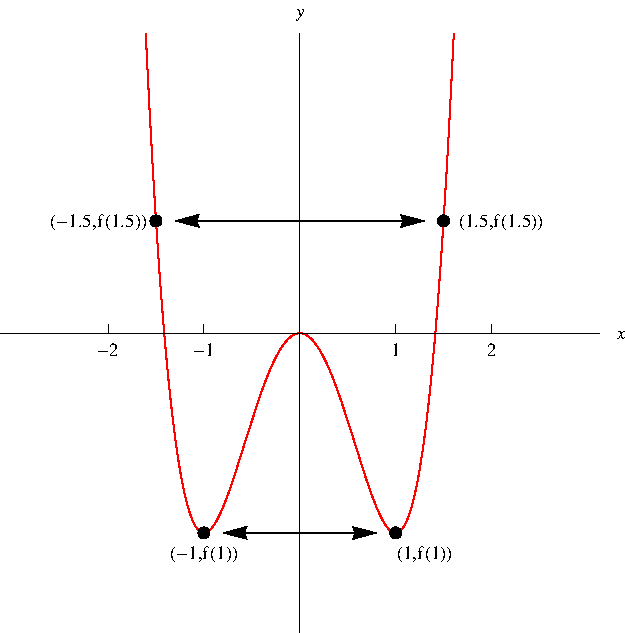
\includegraphics[height=5cm]{curve-sketching/pictures/01-01-even.pdf}%
%}}%
%\only<handout:2| 3>{%
%\ 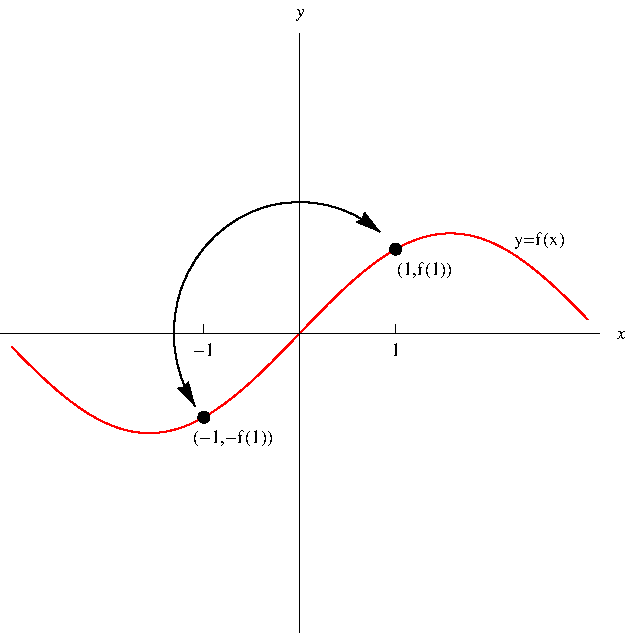
\includegraphics[height=5cm]{curve-sketching/pictures/01-01-odd.pdf}%
%}%
%\only<handout:3| 4->{%
%\ 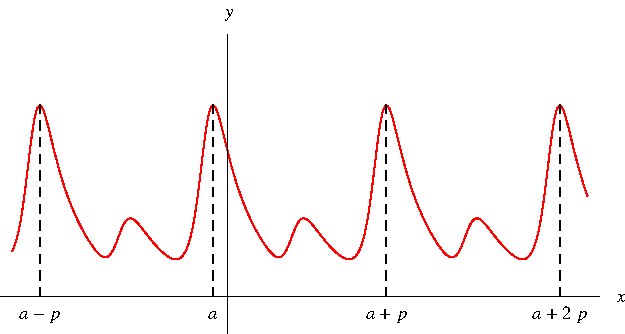
\includegraphics[height=5cm]{curve-sketching/pictures/04-05-periodic.pdf}%
%}
\end{center}
\end{frame}


\begin{frame}[t]
\begin{enumerate}
\setcounter{enumi}{4}
\item  Asymptotes
\end{enumerate}
\begin{itemize}
\item  \textbf{Horizontal asymptotes} can be found by finding $\lim\limits_{x\to\infty} f(x)$ and $\lim\limits_{x\to -\infty} f(x)$.
\item  If either of these equals a number $L$, then $y = L$ is a horizontal asymptote of $f$.  
\item  If neither limit exists, there is no horizontal asymptote.
\item  The line $x = a$ is a \textbf{Vertical asymptote} of $f$ if any of the following is true
\end{itemize}
\[
\begin{array}{ll}
\displaystyle \lim_{x\to a^+}f(x) = \infty &%
\displaystyle \lim_{x\to a^-}f(x) = \infty \\%
\displaystyle \lim_{x\to a^+}f(x) = -\infty &%
\displaystyle \lim_{x\to a^-}f(x) = -\infty %
\end{array}
\]
\begin{itemize}
\item  We may discuss slant asymptotes in another lecture if time allows.
\end{itemize}
\end{frame}


\begin{frame}[t]
\begin{enumerate}
\setcounter{enumi}{5}
\item  Intervals of increase or decrease
\end{enumerate}
\begin{itemize}
\item  To find intervals of increase or decrease, use the increasing/decreasing test.
\item  Compute $f'$.
\item  Find where $f'$ is positive or negative.
\item  Where $f'$ is positive, $f$ is increasing.
\item  Where $f'$ is negative, $f$ is decreasing.
\end{itemize}
\end{frame}




\begin{frame}[t]
\begin{enumerate}
\setcounter{enumi}{6}
\item  Local maxima and minima
\end{enumerate}
\begin{itemize}
\item  Find the critical numbers of $f$ (the numbers $c$ where $f'(c)$ doesn't exist or $f'(c) = 0$).
\item  Use the First Derivative Test on each of these numbers:
\item  If $f'$ changes from positive to negative at a critical number $c$, then $c$ is a local maximum.
\item  If $f'$ changes from negative to positive at a critical number $c$, then $c$ is a local minimum.
\item  If $f'$ doesn't change sign at a critical number $c$, then $c$ is neither a local maximum nor a local minimum.
\end{itemize}
\end{frame}



\begin{frame}[t]
\begin{enumerate}
\setcounter{enumi}{7}
\item  Concavity and points of inflection
\end{enumerate}
\begin{itemize}
\item  To find inflection points and intervals of concavity, use the concavity test.
\item  Compute $f''$.
\item  Find where $f''$ is positive or negative.
\item  Where $f''$ is positive, $f$ is concave up.
\item  Where $f''$ is negative, $f$ is concave down.
\item  Inflection points occur when $f''$ changes signs.
\end{itemize}
\end{frame}
% end module curve-sketching-guidelines

% begin module curve-sketching-guidelines-ex1
\begin{frame}[t]
\begin{example} %[Example 1, p. 245]
\begin{columns}[t]
\column{.45\textwidth}
Sketch the curve $y = \frac{2x^2}{\alertNoH{ 3}{x^2-1}}$.
%\ 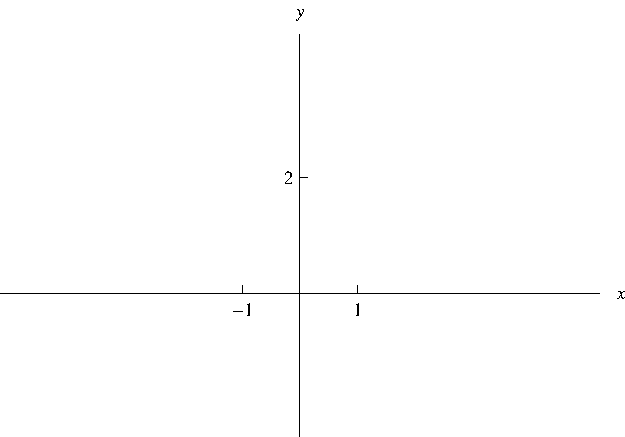
\includegraphics[width=5cm]{curve-sketching/pictures/04-05-ex1a.pdf}%
\psset{xunit=0.25cm, yunit=0.25cm}
\begin{pspicture}(-10,-5.5)(10.5,9)
\psframe*[linecolor=white](-10,-5.5)(10.5,9)
\tiny
\psaxes[ticks=none, labels=none]{<->}(0,0)(-10,-5.5)(10,8.5)
\psline[linecolor=red!1](1,9)(1,9.001)
\psline[linecolor=red!1](1,-5.2)(1,-5.201)

\fcLabels{10}{8.5}
\fcXTickWithLabel{1}{$1$}
\fcXTickWithLabel{-1}{$-1$}
\fcYTickWithLabel{2}{$2$}
\psline[linecolor=red!1](1,9)(1,9.001)
%Function formula: \frac{2 x^{2}}{x^{2}-1}
%\psplot[linecolor=\fcColorGraph, plotpoints=1000]{1.15}{9.9}{x 2 exp 2 mul -1 x 2 exp add div }
%\psplot[linecolor=\fcColorGraph, plotpoints=1000]{-0.85}{0.85}{x 2 exp 2 mul -1 x 2 exp add div }
%\psplot[linecolor=\fcColorGraph, plotpoints=1000]{-9.9}{-1.15}{x 2 exp 2 mul -1 x 2 exp add div }
\end{pspicture}

\invisible<1->{
\abovedisplayskip=0pt
\belowdisplayskip=0pt
\[
\begin{array}{|@{}c@{}|c@{}|c@{}|}
\hline
\textrm{Interval}&\textrm{I/D}&\textrm{Concavity}\\
\hline
(-\infty , -1)&%
\textrm{I}&\\%
(-1 , 0)&%
\textrm{D}&\\%
(0 , 1)&%
\textrm{D}&\\%
(1 , \infty)&%
\textrm{I}&\\%
\hline
\end{array}
\]
}
\column{.55\textwidth}
\begin{enumerate}
\item<2->  Domain
\end{enumerate}
\uncover<2->{%
The domain of the function is \uncover<3->{\alertNoH{ 3}{$(-\infty , -1) \cup (-1, 1)\cup (1,\infty )$}.}
}%
\end{columns}
\end{example}
\end{frame}


\begin{frame}[t]
\begin{example} %[Example 1, p. 245]
\begin{columns}[t]
\column{.45\textwidth}
Sketch the curve $y = \frac{2x^2}{x^2-1}$.
\psset{xunit=0.25cm, yunit=0.25cm}
\begin{pspicture}(-10,-5.5)(10.5,9)
\psframe*[linecolor=white](-10,-5.5)(10.5,9)
\tiny
\psaxes[ticks=none, labels=none]{<->}(0,0)(-10,-5.5)(10,8.5)
\psline[linecolor=red!1](1,9)(1,9.001)
\psline[linecolor=red!1](1,-5.2)(1,-5.201)

\fcLabels{10}{8.5}
\fcXTickWithLabel{1}{$1$}
\fcXTickWithLabel{-1}{$-1$}
\fcYTickWithLabel{2}{$2$}
\uncover<7->{
\fcFullDot{0}{0}
}
\end{pspicture}
%\ \only<handout:0| -5>{%
%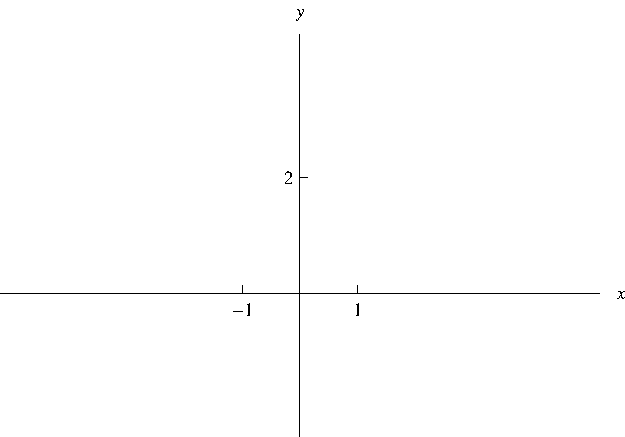
\includegraphics[width=5cm]{curve-sketching/pictures/04-05-ex1a.pdf}%
%}%
%\only<6->{%
%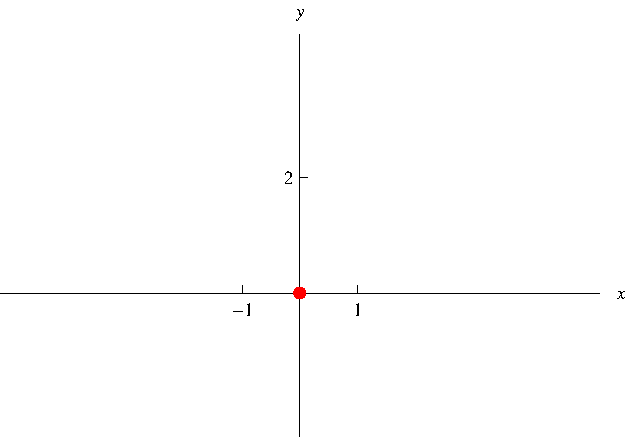
\includegraphics[width=5cm]{curve-sketching/pictures/04-05-ex1b.pdf}%
%}%

\invisible<1->{
\abovedisplayskip=0pt
\belowdisplayskip=0pt
\[
\begin{array}{|@{}c@{}|c@{}|c@{}|}
\hline
\textrm{Interval}&\textrm{I/D}&\textrm{Concavity}\\
\hline
(-\infty , -1)&%
\textrm{I}&\\%
(-1 , 0)&%
\textrm{D}&\\%
(0 , 1)&%
\textrm{D}&\\%
(1 , \infty)&%
\textrm{I}&\\%
\hline
\end{array}
\]
}
\column{.55\textwidth}
\begin{enumerate}
\setcounter{enumi}{2}
\item  Intercepts
\end{enumerate}
\begin{itemize}
\item<2-| alert@2-3>  $y$-intercept: $f(0) = $ \uncover<3->{$0$.}
\item<2-| alert@4-5>  $x$-intercept: $f(x) = 0$ when $x = $ \uncover<5->{$0$.}
\item<6->  The only intercept is $\alertNoH{7}{(0,0)}$.
\end{itemize}
\end{columns}
\end{example}
\end{frame}


\begin{frame}[t]
\begin{example} %[Example 1, p. 245]
\begin{columns}[t]
\column{.45\textwidth}
Sketch the curve $y = \frac{2x^2}{x^2-1}$.
\psset{xunit=0.25cm, yunit=0.25cm}
\begin{pspicture}(-10,-5.5)(10.5,9)
\psframe*[linecolor=white](-10,-5.5)(10.5,9)
\tiny
\psaxes[ticks=none, labels=none]{<->}(0,0)(-10,-5.5)(10,8.5)
\psline[linecolor=red!1](1,9)(1,9.001)
\psline[linecolor=red!1](1,-5.2)(1,-5.201)

\fcLabels{10}{8.5}
\fcXTickWithLabel{1}{$1$}
\fcXTickWithLabel{-1}{$-1$}
\fcYTickWithLabel{2}{$2$}
\fcFullDot{0}{0}
\end{pspicture}

%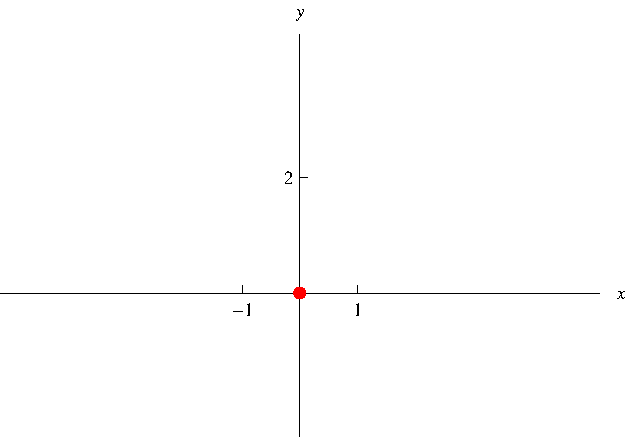
\includegraphics[width=5cm]{curve-sketching/pictures/04-05-ex1b.pdf}%

\invisible<1->{
\abovedisplayskip=0pt
\belowdisplayskip=0pt
\[
\begin{array}{|@{}c@{}|c@{}|c@{}|}
\hline
\textrm{Interval}&\textrm{I/D}&\textrm{Concavity}\\
\hline
(-\infty , -1)&%
\textrm{I}&\\%
(-1 , 0)&%
\textrm{D}&\\%
(0 , 1)&%
\textrm{D}&\\%
(1 , \infty)&%
\textrm{I}&\\%
\hline
\end{array}
\]
}
\column{.55\textwidth}
\begin{enumerate}
\setcounter{enumi}{3}
\item  Symmetry
\end{enumerate}
\[
\uncover<2->{%
f(-x) = \alertNoH{ 3-4}{\frac{2(-x)^2}{(-x)^2-1}} %
}%
\uncover<3->{%
\alertNoH{ 3-4}{ = \uncover<4->{\frac{2x^2}{x^2-1}}} %
}%
\uncover<5->{%
 = f(x)
}%
\]
\uncover<6->{Therefore $f$ is \uncover<7->{\alertNoH{ 7}{even}.}}
\end{columns}
\end{example}
\end{frame}


\begin{frame}[t]
\begin{example} %[Example 1, p. 245]
\begin{columns}[t]
\column{.45\textwidth}
Sketch the curve $y = \frac{2x^2}{x^2-1}$.
\psset{xunit=0.25cm, yunit=0.25cm}
\begin{pspicture}(-10,-5.5)(10.5,9)
\psframe*[linecolor=white](-10,-5.5)(10.5,9)
\tiny
\psaxes[ticks=none, labels=none]{<->}(0,0)(-10,-5.5)(10,8.5)
\psline[linecolor=red!1](1,9)(1,9.001)
\psline[linecolor=red!1](1,-5.2)(1,-5.201)

\fcLabels{10}{8.5}
\uncover<1-14>{
\fcXTickWithLabel{1}{$1$}
\fcXTickWithLabel{-1}{$-1$}
}
\uncover<1-4>{
\fcYTickWithLabel{2}{$2$}
}
\fcFullDot{0}{0}
\uncover<5->{
\psline[linestyle=dashed, linewidth=0.3pt](-9.97,2 )(9.97,2)
\rput[t](-8.5, 1.9){$y=2$}
}
\uncover<4->{ %
\psplot[arrows=->,linecolor=\fcColorGraph, plotpoints=1000]{8}{9.9}{x 2 exp 2 mul -1 x 2 exp add div }
} %
\uncover<8->{ %
\psplot[arrows=<-,linecolor=\fcColorGraph, plotpoints=1000]{1.2}{1.8}{x 2 exp 2 mul -1 x 2 exp add div }
} %
\uncover<10->{
\psplot[arrows=->, linecolor=\fcColorGraph, plotpoints=1000]{0.65}{0.8}{x 2 exp 2 mul -1 x 2 exp add div }
}
\uncover<12->{
\psplot[arrows=<-, linecolor=\fcColorGraph, plotpoints=1000]{-0.8}{-0.65}{x 2 exp 2 mul -1 x 2 exp add div }
}

\uncover<4->{ %
\psplot[arrows=<-, linecolor=\fcColorGraph, plotpoints=1000]{-9.9}{-8}{x 2 exp 2 mul -1 x 2 exp add div }
} %
\uncover<14->{ %
\psplot[arrows=->, linecolor=\fcColorGraph, plotpoints=1000]{-1.8}{-1.2}{x 2 exp 2 mul -1 x 2 exp add div }
} %
\uncover<15->{ %
\psline[linestyle=dashed, linewidth=0.3pt](-1,-5)(-1,8)
\rput[r](-1.4, -3.5){$x=-1$}
\psline[linestyle=dashed, linewidth=0.3pt](1,-5)(1,8)
\rput[l](1.4, -3.5){$x=1$}
} %
\end{pspicture}

%\ \only<handout:0| -3>{%
%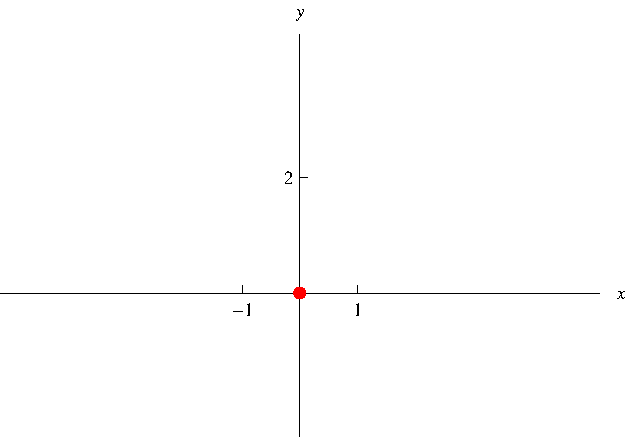
\includegraphics[width=5cm]{curve-sketching/pictures/04-05-ex1b.pdf}%
%}%
%\only<handout:0| 4>{%
%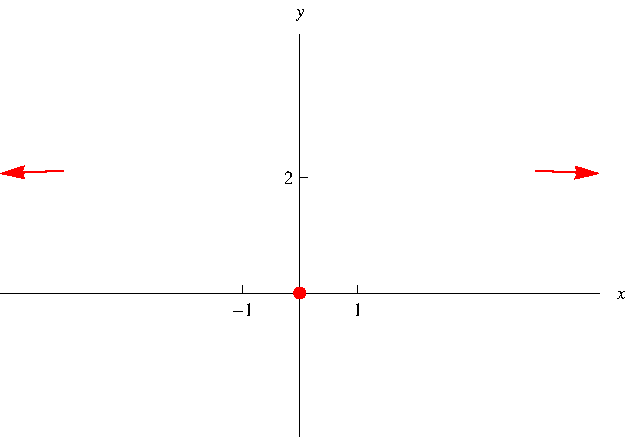
\includegraphics[width=5cm]{curve-sketching/pictures/04-05-ex1c.pdf}%
%}%
%\only<handout:0| 5-7>{%
%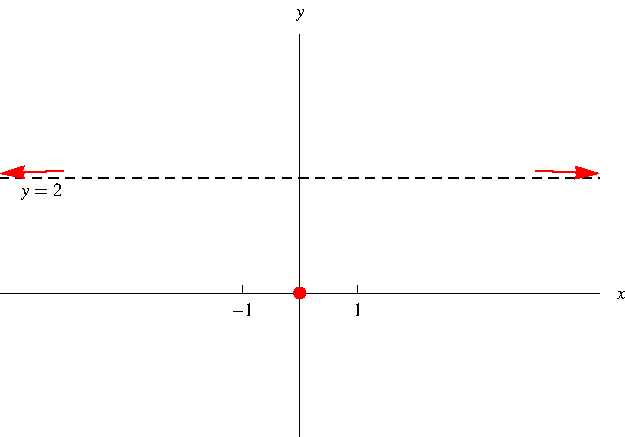
\includegraphics[width=5cm]{curve-sketching/pictures/04-05-ex1d.pdf}%
%}%
%\only<handout:0| 8-9>{%
%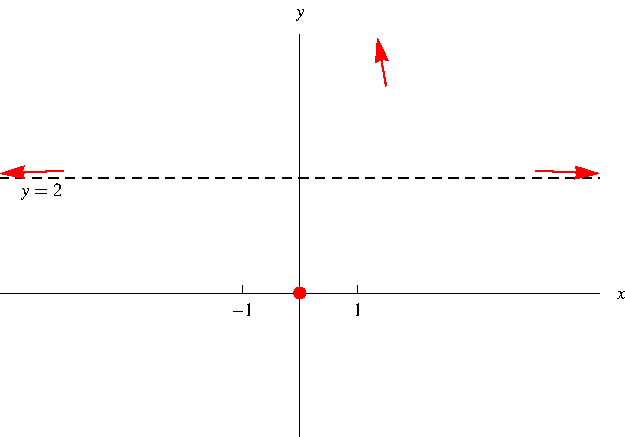
\includegraphics[width=5cm]{curve-sketching/pictures/04-05-ex1e.pdf}%
%}%
%\only<handout:0| 10-11>{%
%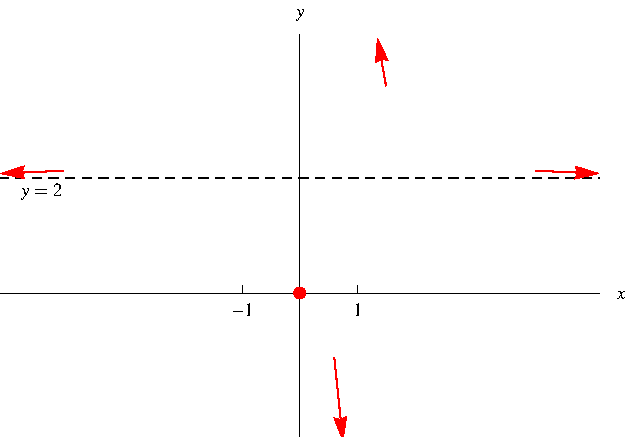
\includegraphics[width=5cm]{curve-sketching/pictures/04-05-ex1f.pdf}%
%}%
%\only<handout:0| 12-13>{%
%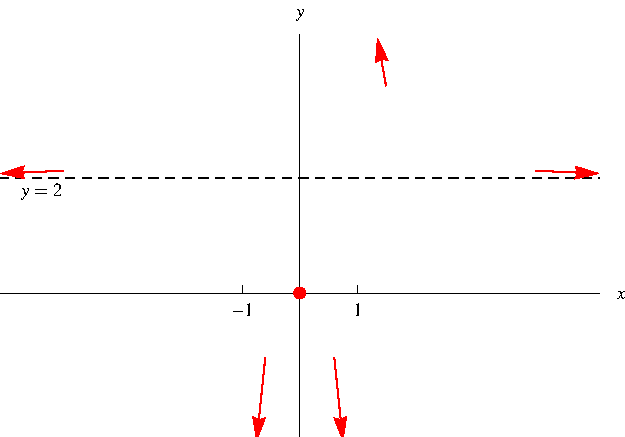
\includegraphics[width=5cm]{curve-sketching/pictures/04-05-ex1g.pdf}%
%}%
%\only<handout:0| 14>{%
%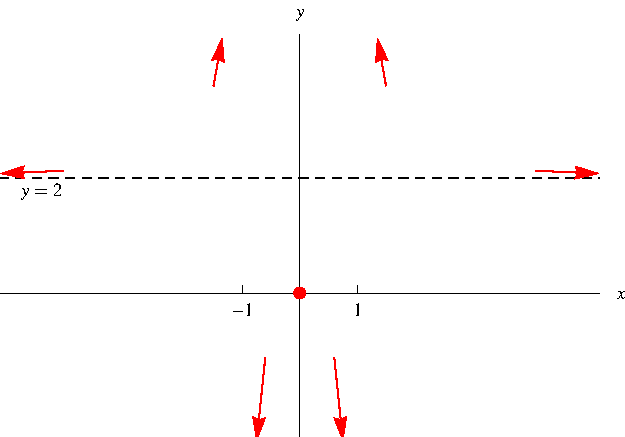
\includegraphics[width=5cm]{curve-sketching/pictures/04-05-ex1h.pdf}%
%}%
%\only<15->{%
%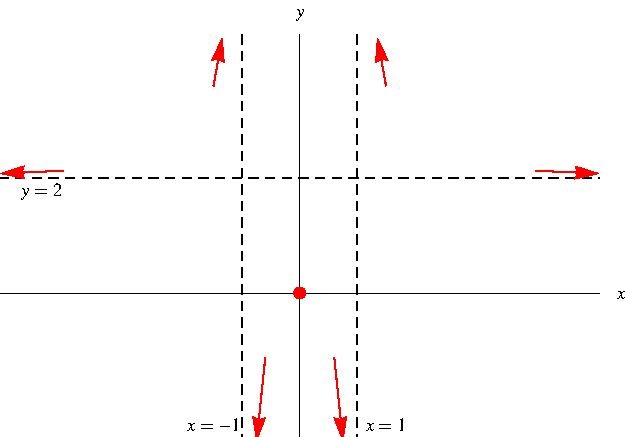
\includegraphics[width=5cm]{curve-sketching/pictures/04-05-ex1i.pdf}%
%}%

\invisible<1->{
\abovedisplayskip=0pt
\belowdisplayskip=0pt
\[
\begin{array}{|@{}c@{}|c@{}|c@{}|}
\hline
\textrm{Interval}&\textrm{I/D}&\textrm{Concavity}\\
\hline
(-\infty , -1)&%
\textrm{I}&\\%
(-1 , 0)&%
\textrm{D}&\\%
(0 , 1)&%
\textrm{D}&\\%
(1 , \infty)&%
\textrm{I}&\\%
\hline
\end{array}
\]
}

\column{.55\textwidth}
\begin{enumerate}
\setcounter{enumi}{4}
\item  Asymptotes
\end{enumerate}
\abovedisplayskip=0pt
\belowdisplayskip=0pt
\[
\uncover<2->{%
\lim_{x\to\pm\infty}\frac{2x^2}{x^2-1}%
}%
\uncover<3->{%
 = \lim_{x\to\pm\infty}\frac{2}{1 - 1/x^2}%
}%
\uncover<4->{%
 = 2%
}%
\]
\uncover<5->{$y = 2$ is a horizontal asymptote.}
\uncover<6->{%
\abovedisplayskip=0pt
\belowdisplayskip=0pt
\[
\begin{array}{r@{}c@{}l}
\displaystyle \alertNoH{ 7-8}{\lim_{x\to 1^+}\frac{2x^2}{x^2-1}} & \alertNoH{ 7-8}{=} & \uncover<8->{\alertNoH{ 8}{\infty}} \\%
\displaystyle \alertNoH{ 9-10}{\lim_{x\to 1^-}\frac{2x^2}{x^2-1}} & \alertNoH{ 9-10}{=} & \uncover<10->{\alertNoH{ 10}{-\infty}} \\%
\displaystyle \alertNoH{ 11-12}{\lim_{x\to -1^+}\frac{2x^2}{x^2-1}} & \alertNoH{ 11-12}{=} & \uncover<12->{\alertNoH{ 12}{-\infty}} \\%
\displaystyle \alertNoH{ 13-14}{\lim_{x\to -1^-}\frac{2x^2}{x^2-1}} & \alertNoH{ 13-14}{=} & \uncover<14->{\alertNoH{ 14}{\infty}} %
\end{array}
\]
}%
\uncover<15->{%
$x = \pm 1$ are vertical asymptotes.%
}%
\end{columns}
\end{example}
\end{frame}


\begin{frame}[t]
\begin{example} %[Example 1, p. 245]
\begin{columns}[t]
\column{.45\textwidth}
Sketch the curve $y = \frac{2x^2}{x^2-1}$.
\psset{xunit=0.25cm, yunit=0.25cm}
\begin{pspicture}(-10,-5.5)(10.5,9)
\psframe*[linecolor=white](-10,-5.5)(10.5,9)
\tiny
\psaxes[ticks=none, labels=none]{<->}(0,0)(-10,-5.5)(10,8.5)
\psline[linecolor=red!1](1,9)(1,9.001)
\psline[linecolor=red!1](1,-5.2)(1,-5.201)

\fcLabels{10}{8.5}
\fcFullDot{0}{0}
\psline[linestyle=dashed, linewidth=0.3pt](-9.97,2 )(9.97,2)
\rput[t](-8.5, 1.9){$y=2$}
\psplot[arrows=->,linecolor=\fcColorGraph, plotpoints=1000]{8}{9.9}{x 2 exp 2 mul -1 x 2 exp add div }
\psplot[arrows=<-,linecolor=\fcColorGraph, plotpoints=1000]{1.2}{1.8}{x 2 exp 2 mul -1 x 2 exp add div }
\psplot[arrows=->, linecolor=\fcColorGraph, plotpoints=1000]{0.65}{0.8}{x 2 exp 2 mul -1 x 2 exp add div }
\psplot[arrows=<-, linecolor=\fcColorGraph, plotpoints=1000]{-0.8}{-0.65}{x 2 exp 2 mul -1 x 2 exp add div }
\psplot[arrows=<-, linecolor=\fcColorGraph, plotpoints=1000]{-9.9}{-8}{x 2 exp 2 mul -1 x 2 exp add div }
\psplot[arrows=->, linecolor=\fcColorGraph, plotpoints=1000]{-1.8}{-1.2}{x 2 exp 2 mul -1 x 2 exp add div }
\psline[linestyle=dashed, linewidth=0.3pt](-1,-5)(-1,8)
\rput[r](-1.4, -3.5){$x=-1$}
\psline[linestyle=dashed, linewidth=0.3pt](1,-5)(1,8)
\rput[l](1.4, -3.5){$x=1$}
\end{pspicture}

%\ \only<1->{%
%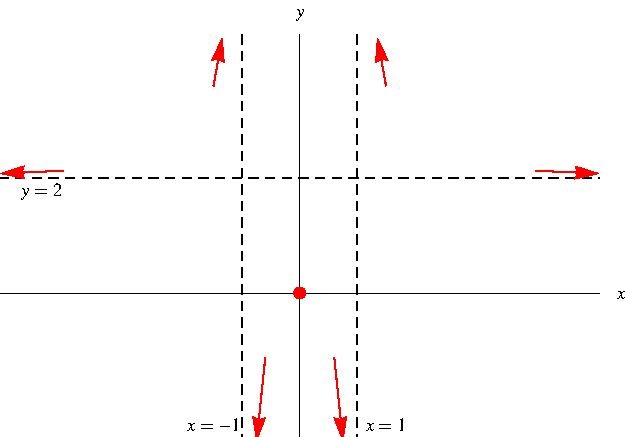
\includegraphics[width=5cm]{curve-sketching/pictures/04-05-ex1i.pdf}%
%}%

\abovedisplayskip=0pt
\belowdisplayskip=0pt
\[
\begin{array}{|@{}c@{}|c@{}|c@{}|}
\hline
\textrm{Interval}&\alertNoH{ 12}{\textrm{I/D}}&\textrm{Concavity}\\
\hline
(-\infty , -1)&%
\uncover<12->{\alertNoH{ 12}{\textrm{I}}}&\\%
(-1 , 0)&%
\uncover<12->{\alertNoH{ 12}{\textrm{I}}}&\\%
(0 , 1)&%
\uncover<12->{\alertNoH{ 12}{\textrm{D}}}&\\%
(1 , \infty)&%
\uncover<12->{\alertNoH{ 12}{\textrm{D}}}&\\%
\hline
\end{array}
\]

\column{.55\textwidth}
\begin{enumerate}
\setcounter{enumi}{5}
\item  Intervals of increase or decrease
\end{enumerate}
\abovedisplayskip=0pt
\belowdisplayskip=0pt
\begin{eqnarray*}
\uncover<2->{%
\alertNoH{ 3-4}{f'(x)}%
}%
& \uncover<2->{\alertNoH{ 3-4}{ = }} &%
\uncover<4->{%
\alertNoH{ 4}{\frac{(x^2-1)(4x) - 2x^2(2x)}{(x^2-1)^2}}%
}\\%
&\uncover<5->{ = } &%
\uncover<5->{%
 \frac{-4x}{(x^2-1)^2}%
}%
\end{eqnarray*}
\uncover<6->{%
\[
\begin{array}{|c@{}|c@{}|c@{}|c@{}|}
\hline
& \alertNoH{ 7-8}{-4x} & \alertNoH{ 9-10}{(x^2-1)^2} & \alertNoH{ 11}{f'} \\
\hline
(-\infty , -1) & \alertNoH{ 7-8}{\uncover<8->{+}} & \alertNoH{ 9-10}{\uncover<10->{+}} & \alertNoH{ 11}{\uncover<11->{+}} \\
(-1 , 0) & \alertNoH{ 7-8}{\uncover<8->{+}} & \alertNoH{ 9-10}{\uncover<10->{+}} & \alertNoH{ 11}{\uncover<11->{+}} \\
(0 , 1) & \alertNoH{ 7-8}{\uncover<8->{-}} & \alertNoH{ 9-10}{\uncover<10->{+}} & \alertNoH{ 11}{\uncover<11->{-}} \\
(1 , \infty) & \alertNoH{ 7-8}{\uncover<8->{-}} & \alertNoH{ 9-10}{\uncover<10->{+}} & \alertNoH{ 11}{\uncover<11->{-}} \\
\hline
\end{array}
\]
}%
\end{columns}
\end{example}
\end{frame}


\begin{frame}[t]
\begin{example} %[Example 1, p. 245]
\begin{columns}[t]
\column{.45\textwidth}
Sketch the curve $y = \frac{2x^2}{x^2-1}$.
\psset{xunit=0.25cm, yunit=0.25cm}
\begin{pspicture}(-10,-5.5)(10.5,9)
\psframe*[linecolor=white](-10,-5.5)(10.5,9)
\tiny
\psaxes[ticks=none, labels=none]{<->}(0,0)(-10,-5.5)(10,8.5)
\psline[linecolor=red!1](1,9)(1,9.001)
\psline[linecolor=red!1](1,-5.2)(1,-5.201)

\fcLabels{10}{8.5}
\fcFullDot{0}{0}
\psline[linestyle=dashed, linewidth=0.3pt](-9.97,2 )(9.97,2)
\rput[t](-8.5, 1.9){$y=2$}
\psplot[arrows=->,linecolor=\fcColorGraph, plotpoints=1000]{8}{9.9}{x 2 exp 2 mul -1 x 2 exp add div }
\psplot[arrows=<-,linecolor=\fcColorGraph, plotpoints=1000]{1.2}{1.8}{x 2 exp 2 mul -1 x 2 exp add div }
\psplot[arrows=->, linecolor=\fcColorGraph, plotpoints=1000]{0.65}{0.8}{x 2 exp 2 mul -1 x 2 exp add div }
\psplot[arrows=<-, linecolor=\fcColorGraph, plotpoints=1000]{-0.8}{-0.65}{x 2 exp 2 mul -1 x 2 exp add div }
\psplot[arrows=<-, linecolor=\fcColorGraph, plotpoints=1000]{-9.9}{-8}{x 2 exp 2 mul -1 x 2 exp add div }
\psplot[arrows=->, linecolor=\fcColorGraph, plotpoints=1000]{-1.8}{-1.2}{x 2 exp 2 mul -1 x 2 exp add div }
\psline[linestyle=dashed, linewidth=0.3pt](-1,-5)(-1,8)
\rput[r](-1.4, -3.5){$x=-1$}
\psline[linestyle=dashed, linewidth=0.3pt](1,-5)(1,8)
\rput[l](1.4, -3.5){$x=1$}
\end{pspicture}

%\ \only<1->{%
%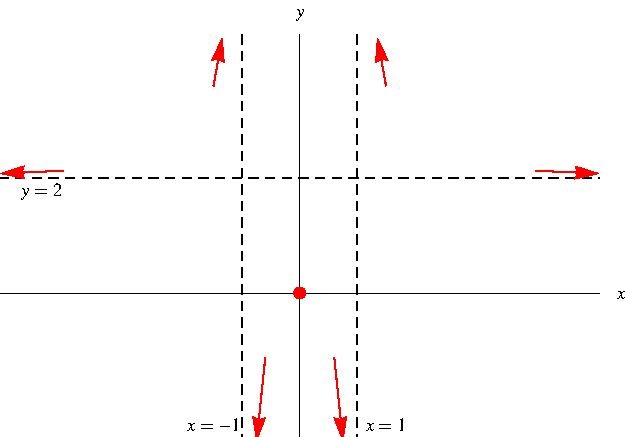
\includegraphics[width=5cm]{curve-sketching/pictures/04-05-ex1i.pdf}%
%}%

\abovedisplayskip=0pt
\belowdisplayskip=0pt
\[
\begin{array}{|@{}c@{}|c@{}|c@{}|}
\hline
\textrm{Interval}&\textrm{I/D}&\textrm{Concavity}\\
\hline
(-\infty , -1)&%
\textrm{I}&\\%
(-1 , 0)&%
\textrm{I}&\\%
(0 , 1)&%
\textrm{D}&\\%
(1 , \infty)&%
\textrm{D}&\\%
\hline
\end{array}
\]

\column{.55\textwidth}
\begin{enumerate}
\setcounter{enumi}{6}
\item  Local maxima and minima
\end{enumerate}
\[
\begin{array}{|c@{}|c@{}|c@{}|c@{}|}
\hline
& -4x & (x^2-1)^2 & f' \\
\hline
(-\infty , -1) & + & + & + \\
\alertNoH{ 2}{(-1 , 0)} & + & + & \alertNoH{ 2}{+} \\
\alertNoH{ 2}{(0 , 1)} & - & + & \alertNoH{ 2}{-} \\
(1 , \infty) & - & + & - \\
\hline
\end{array}
\]
\begin{itemize}
\item<2->  $f'$ changes sign from $+$ to $-$ at $0$.
\item<3->  Therefore $(0,0)$ is a local maximum.
\end{itemize}
\end{columns}
\end{example}
\end{frame}

\begin{frame}[t]
\begin{example} %[Example 1, p. 245]
\begin{columns}[t]
\column{.45\textwidth}
Sketch the curve $y = \frac{2x^2}{x^2-1}$.
\psset{xunit=0.25cm, yunit=0.25cm}
\begin{pspicture}(-10,-5.5)(10.5,9)
\psframe*[linecolor=white](-10,-5.5)(10.5,9)
\tiny
\psaxes[ticks=none, labels=none]{<->}(0,0)(-10,-5.5)(10,8.5)
\psline[linecolor=red!1](1,9)(1,9.001)
\psline[linecolor=red!1](1,-5.2)(1,-5.201)

\fcLabels{10}{8.5}
\fcFullDot{0}{0}
\psline[linestyle=dashed, linewidth=0.3pt](-9.97,2 )(9.97,2)
\rput[t](-8.5, 1.9){$y=2$}
\psline[linestyle=dashed, linewidth=0.3pt](-1,-5)(-1,8)
\rput[r](-1.4, -3.5){$x=-1$}
\psline[linestyle=dashed, linewidth=0.3pt](1,-5)(1,8)
\rput[l](1.4, -3.5){$x=1$}
\uncover<1-13>{ %
\psplot[arrows=->,linecolor=\fcColorGraph, plotpoints=1000]{8}{9.9}{x 2 exp 2 mul -1 x 2 exp add div }
\psplot[arrows=<-,linecolor=\fcColorGraph, plotpoints=1000]{1.2}{1.8}{x 2 exp 2 mul -1 x 2 exp add div }
\psplot[arrows=->, linecolor=\fcColorGraph, plotpoints=1000]{0.65}{0.8}{x 2 exp 2 mul -1 x 2 exp add div }
\psplot[arrows=<-, linecolor=\fcColorGraph, plotpoints=1000]{-0.8}{-0.65}{x 2 exp 2 mul -1 x 2 exp add div }
\psplot[arrows=<-, linecolor=\fcColorGraph, plotpoints=1000]{-9.9}{-8}{x 2 exp 2 mul -1 x 2 exp add div }
\psplot[arrows=->, linecolor=\fcColorGraph, plotpoints=1000]{-1.8}{-1.2}{x 2 exp 2 mul -1 x 2 exp add div }
}
\uncover<14->{ %
\psplot[linecolor=\fcColorGraph, plotpoints=1000]{1.15}{9.9}{x 2 exp 2 mul -1 x 2 exp add div }
\psplot[linecolor=\fcColorGraph, plotpoints=1000]{-0.85}{0.85}{x 2 exp 2 mul -1 x 2 exp add div }
\psplot[linecolor=\fcColorGraph, plotpoints=1000]{-9.9}{-1.15}{x 2 exp 2 mul -1 x 2 exp add div }
} %
\end{pspicture}
%\ \only<handout:0| -13>{%
%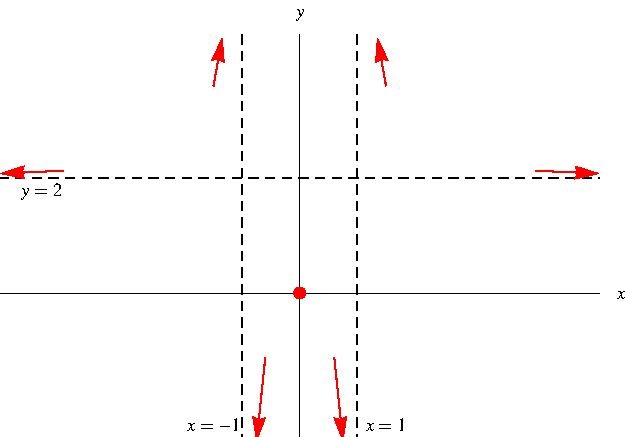
\includegraphics[width=5cm]{curve-sketching/pictures/04-05-ex1i.pdf}%
%}%
%\only<14->{%
%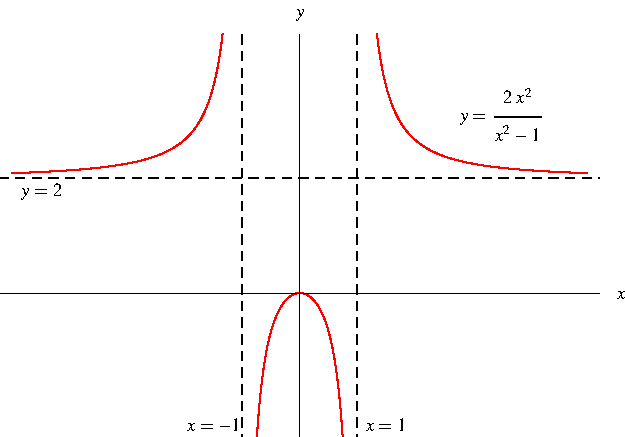
\includegraphics[width=5cm]{curve-sketching/pictures/04-05-ex1j.pdf}%
%}%

\abovedisplayskip=0pt
\belowdisplayskip=0pt
\[
\begin{array}{|@{}c@{}|c@{}|c@{}|}
\hline
\textrm{Interval}&\textrm{I/D}&\alertNoH{ 12}{\textrm{Concavity}}\\
\hline
(-\infty , -1)&%
\textrm{I}&\uncover<12->{\alertNoH{ 12}{\textrm{up}}}\\%
(-1 , 0)&%
\textrm{I}&\uncover<12->{\alertNoH{ 12}{\textrm{down}}}\\%
(0 , 1)&%
\textrm{D}&\uncover<12->{\alertNoH{ 12}{\textrm{down}}}\\%
(1 , \infty)&%
\textrm{D}&\uncover<12->{\alertNoH{ 12}{\textrm{up}}}\\%
\hline
\end{array}
\]

\column{.55\textwidth}
\begin{enumerate}
\setcounter{enumi}{7}
\item  Concavity and points of inflection
\end{enumerate}
\abovedisplayskip=0pt
\belowdisplayskip=0pt
\begin{eqnarray*}
& & \uncover<2->{%
\ \ \alertNoH{ 3-4}{f''(x)}%
}\\%
%& \uncover<2->{\alertNoH{ 3-4}{ = }} &%
&&\uncover<4->{%
\alertNoH{ 4}{ = \frac{-4(x^2-1)^2+4x\cdot 2(x^2-1)2x}{(x^2-1)^4}}%
}\\%
%&\uncover<5->{ = } &%
&&\uncover<5->{%
 =  \frac{12x^2+4}{(x^2-1)^3}%
}%
\end{eqnarray*}
\uncover<6->{%
\[
\begin{array}{|@{}c@{}|c@{}|c@{}|c@{}|}
\hline
& \alertNoH{ 7-8}{12x^2+4} & \alertNoH{ 9-10}{(x^2-1)^3} & \alertNoH{ 11}{f''} \\
\hline
(-\infty , -1) & \alertNoH{ 7-8}{\uncover<8->{+}} & \alertNoH{ 9-10}{\uncover<10->{+}} & \alertNoH{ 11}{\uncover<11->{+}} \\
(-1 , 1) & \alertNoH{ 7-8}{\uncover<8->{+}} & \alertNoH{ 9-10}{\uncover<10->{-}} & \alertNoH{ 11}{\uncover<11->{-}} \\
(1 , \infty) & \alertNoH{ 7-8}{\uncover<8->{+}} & \alertNoH{ 9-10}{\uncover<10->{+}} & \alertNoH{ 11}{\uncover<11->{+}} \\
\hline
\end{array}
\]
}%
\uncover<13,14->{%
No points of inflection because $\pm 1$ are not in the domain of $f$.
}%
\end{columns}
\end{example}
\end{frame}
% end module curve-sketching-guidelines-ex1

% end lecture

\end{document}
